\section{分级复核与保守修正}
\label{sec:gating}

候选级复核同时受到调用成本与修改风险的约束。对全部候选调用多模态大模型会使计算开销随候选数线性增长。若直接用模型结论覆盖检测结果，错误判断还会抵消基础检测器的性能。本文用四个模块分离调用选择、候选验证、动作映射和动作执行权限。复核调用选择门 M6 简称复检门，只决定哪些候选进入多模态验证器。多模态验证器 M8 给出独立视觉结论，M9 将结论映射为提议动作，接受门 M10 判断是否执行。复检门优化有限预算下的错误覆盖，接受门约束修改风险，二者不能由同一阈值替代。

\subsection{复检门（M6）}
\label{subsec:review-gate}

设候选 $x_i$ 的基础检测结果及外部证据特征为 $z_i^{\mathrm{review}}$。复检门不判断候选处是否存在缺陷。其监督目标是预测该候选是否包含可由多模态验证器处理且有可执行修正动作的错误：
\begin{equation}
 y_i^{\mathrm{review}}=
 \mathbb{I}\!\left[x_i\text{ 对应可修复的误报、漏检或错分类}\right].
 \label{eq:review-label}
\end{equation}
该定义区分“困难样本”和“可修复错误”。低置信度的正确检测不应占用有限调用预算。高置信度误报和差异分支发现的漏检候选则是正例的主要来源。复检门输出风险分数 $r_i=g_r(z_i^{\mathrm{review}})$，并在调用率预算 $b$ 下选择分数最高的前 $b$ 比例候选。阈值随预算变化。复检门不读取多模态验证器输出，也不决定检测框的增删改。

输入特征覆盖检测器不确定性、候选来源、参考差异和几何属性。检测器侧使用温度校准后的置信度、类别 margin 与预测熵。来源标记采用 DET、DIFF、BOTH 的独热表示，并保留检测框与差异框的重叠信息。外观证据包括残差均值、95 分位数和超过差异阈值的面积比例。8 维拓扑向量描述连通分量、端点、分支点、欧拉数、骨架长度、拓扑异或面积、区域面积和周长的变化。配准质量 $q_{\mathrm{reg}}$ 表示正常模板证据的可信程度。框宽、框高和长宽比补充尺度信息。特征向量为
\begin{equation}
 z_i^{\mathrm{review}}=[p_i^{cal},m_i,H_i,s_i,u_i^{\mathrm{app}},t_i,q_{\mathrm{reg}},w_i,h_i,w_i/h_i],
 \label{eq:review-features}
\end{equation}
其中 $s_i$ 表示来源及来源间重叠特征，$u_i^{\mathrm{app}}$ 表示外观残差统计，$t_i\in\mathbb{R}^{8}$ 表示拓扑向量。拓扑差异图在证据消融后不再作为多模态验证器的视觉输入，其数值向量仍作为复检门的结构化特征。

本文比较 L2 正则 Logistic 回归与 LightGBM。Logistic 便于解释特征方向，LightGBM 可描述特征间的非线性交互。阶段 C 的五折 OOF 数据包含 51222 个候选，正例率约为 2.1\%。表~\ref{tab:review-gate-models} 给出设计阶段的跨折结果。LightGBM 的 PR AP 为 0.4311，Logistic 为 0.1839，前者约为后者的 2.3 倍。两者的 ROC AUC 分别为 0.9227 和 0.7909。负例占多数时，PR AP 更直接反映少数正例的排序质量。方法上两类模型均可用于复检门。阶段 D 按预注册协议固定使用 Logistic 主模型，LightGBM 仅作对照。本文未依据测试结果更换主模型。完整比较见第~\ref{sec:experiments}章。

\begin{table}[t]
  \centering
  \caption{阶段 C 复检门的五折 OOF 性能}
  \label{tab:review-gate-models}
  \begin{tabular}{lcc}
    \hline
    模型 & PR AP & ROC AUC \\
    \hline
    Logistic & 0.1839 & 0.7909 \\
    LightGBM & \textbf{0.4311} & \textbf{0.9227} \\
    \hline
  \end{tabular}
\end{table}

\subsection{多模态验证器（M8）与动作映射（M9）}
\label{subsec:mllm-action-map}

多模态验证器采用去锚定输入原则。模型查看当前候选紧裁剪、局部上下文和对齐后的正常模板紧裁剪，不读取检测器类别、置信度和系统期望动作。模型先作出视觉判断，系统再将其与检测结果比较。多模态验证器不能在整幅图像中搜索缺陷，只能验证 DET、DIFF 或 BOTH 分支给出的候选区域。该任务属于封闭候选验证。

缺陷类别限于数据集定义的六类。标签为 open、short、mousebite、spur、pinhole 和 spurious\_copper。存在性只能取 true、false 或 null。类别字段在六类之外只允许 normal 与 uncertain。参考可靠性、外观模式、拓扑模式、证据强度和原因码均使用固定枚举。冻结的 JSON Schema 设有 defect\_present 和 predicted\_class 字段。reference\_reliability 记录参考可靠性。appearance\_pattern 与 topology\_pattern 记录两类模式。evidence\_strength 与 reason\_codes 分别记录证据强度和原因码。自由文本对照的 JSON 可解析率为 0.0000，无法稳定支持动作映射、接受特征构造和审计记录。因此主实验采用结构化输出，解析失败或字段越界均标记为无效。系统不从自然语言中猜测动作，完整实验结果见第~\ref{sec:experiments}章。

M9 在多模态验证器外部执行确定性映射，规则见表~\ref{tab:action-map}。DET 和 BOTH 候选包含基础检测框。独立结论为 normal 时提议 remove；结论为缺陷且类别与检测器一致时 keep。只有新类别非 uncertain、拓扑证据支持新类别并反驳原类别时，系统才提议 relabel。无法形成确定结论时 defer。DIFF 候选不依附已有检测框。受支持的缺陷结论映射为 add，normal 映射为 reject，不确定结论映射为 reject 或 defer。BOTH 候选不能通过 add 生成重叠框。多模态验证器只描述视觉结论，系统侧映射保留最终修改权限。

\begin{table}[t]
  \centering
  \caption{候选来源与独立结论的动作映射}
  \label{tab:action-map}
  \begin{tabular}{lll}
    \hline
    来源 & 独立结论 & 提议动作 \\
    \hline
    DET/BOTH & normal & remove \\
    DET/BOTH & 缺陷且类别相同 & keep \\
    DET/BOTH & 缺陷且类别不同、证据一致 & relabel \\
    DET/BOTH & uncertain & defer/keep \\
    DIFF & 缺陷 & add \\
    DIFF & normal & reject \\
    DIFF & uncertain & reject/defer \\
    \hline
  \end{tabular}
\end{table}

动作优先级由五折基础检测错误分解决定。可纠错空间包含漏检 947 个、误报 636 个和错分类 61 个。三者分别占 57.6\%、38.7\% 和 3.7\%。prompt 先判断候选处是否存在受支持缺陷。该判断服务于 DIFF 候选的 add 动作和 DET/BOTH 候选的 remove 动作。relabel 的理论收益上限最小，错误判断还会把位置正确的检测转化为错分类。因此，relabel 同时要求封闭类别、非 uncertain 结论和类别拓扑一致性。该设计按错误构成分配三类动作的判断能力和风险额度，完整错误分解见第~\ref{sec:experiments}章。

prompt 版本实验显示存在性 F1 与 remove 可用性之间存在权衡。v1 的缺陷存在性 F1 为 0.7678，高于 v2 的 0.7347。v1 的 normal 判定率为 0.31，低于 v2 的 0.39。提高 normal 判定率有助于识别误报，但会降低整体存在性 F1。remove 依赖 normal 结论，因为 DET/BOTH 候选只有在模型否定缺陷时才会提出删除。早期开发 smoke 实验中，v1 的 normal 判定率为 0.000，remove 因而不可用。v2 加强 normal 引导并接受存在性 F1 下降，目标是恢复双向纠错能力，而不是证明 v2 全面优于 v1。第~\ref{sec:experiments}章同时报告两个指标，以呈现动作分布的变化。

\subsection{接受门（M10）与安全规则}
\label{subsec:acceptance-gate}

复检门放行只表示候选值得查看，多模态验证器给出提议动作也不表示该动作安全。接受门预测执行每个提议动作是否产生正效用。给定当前预测集合 $\hat{Y}$、真值 $Y^{*}$ 和动作 $a_i$，训练标签定义为
\begin{equation}
 y_i^{\mathrm{accept}}=
 \mathbb{I}\!\left[U(\hat{Y}\oplus a_i,Y^{*})>U(\hat{Y},Y^{*})\right],
 \label{eq:accept-label}
\end{equation}
其中 $\oplus$ 表示执行动作。删除原始误报构成 remove 的正效用标签。将已匹配位置改为正确类别构成 relabel 的正效用标签。添加匹配原漏检真值的差异框构成 add 的正效用标签。损害检测结果或没有改善的修改均为负例。

不同动作的样本机制、风险和正例率不同。因此，接受门按 remove、relabel、add 分开训练，不将动作独热编码后混合拟合。输入先沿用复检特征，再加入多模态验证器的存在性与类别结论。其他输入包括证据强度、参考可靠性、外观一致性、拓扑一致性和 JSON 有效标记。最终执行条件为
\begin{equation}
 \operatorname{Apply}(a_i)=
 \mathbb{I}[g_{a_i}(z_i^{\mathrm{accept}})\geq \tau_{a_i}]
 \land \operatorname{SafetyRule}(a_i),
 \label{eq:accept-rule}
\end{equation}
其中 $g_{a_i}$ 是动作专属接受模型，$\tau_{a_i}$ 是动作阈值。模型概率只提供统计证据，不能绕过硬安全规则。

阶段 C 的五折训练分布支持按动作建模。remove 每折约 800 个样本，正例为 26 到 46 个。add 每折约 12000 个样本，正例为 39 到 55 个。两类数据均高度不平衡，但仍包含正负例。relabel 每折约 2300 个样本，正例仅为 0 到 5 个，fold3 为 0。全数据只有 61 个错分类。折隔离和提议动作筛选后，这些数据无法支持稳定的 relabel 接受模型。类别权重或过采样不能消除这一限制。fold3 的标签单一，因而触发保守退化；relabel 模型不输出接受概率，系统拒绝该动作。其他折即使能够拟合，也必须服从更高阈值和拓扑一致性检查。完整分布见第~\ref{sec:experiments}章。

硬安全规则按动作后果设置。remove 会丢弃已有检测，因而使用三类动作中的最高阈值，且只作用于 DET 或 BOTH 候选。relabel 只能在封闭的六类标签内执行。多模态验证器的类别结论必须与拓扑模式一致，来源也必须包含原检测框。add 只能采用已有 DIFF 候选的确定性边界，不允许多模态验证器生成坐标。BOTH 候选已有检测框，不能执行 add。配准质量 $q_{\mathrm{reg}}$ 低于阈值时，系统禁止 remove、relabel 和 add。在选定平移序列中，$q_{\mathrm{reg}}$ 随扰动增强而总体下降，可用作可靠性指标。但阈值 0.5 拦截的有害动作数为 0。当前实验尚未证实该安全规则的保护作用，详见第~\ref{sec:experiments}章。JSON 解析失败、字段非法或动作冲突时，系统保留基础检测器输出或将候选交由人工处理。

训练不足时，兜底方向决定最坏情况风险。若样本少于最低要求或训练标签单一，接受概率固定回退为 0，并拒绝全部修改。早期实现采用接受式退化，多模态验证器的错误会直接进入最终结果。保守退化则返回未修改基线，并放弃当前数据无法支持的收益。该规则对 relabel 尤其关键，因为 fold3 没有正例。

\subsection{防泄漏与门控训练协议}
\label{subsec:gating-protocol}

数据按 PCB 模板组执行五折 GroupKFold，同一模板的旋转图和衍生图不能跨越训练与测试边界。第 $i$ 折以该折图像为 test，以第 $(i+1)\bmod 5$ 折为 val，其余三折训练检测器。五折本身已经覆盖全部 1500 张图，每张图恰好在一折中作为 test，且产生该图预测的检测器从未见过该图。将五个 test 折的输出拼接即可得到完整 OOF 候选集合，不需要再在每个外层折中嵌套检测器交叉拟合。

若在每个外折内重新构造四折检测器预测，两层折叠需要 20 次训练。本文协议只训练 5 次检测器，同时使每条门控记录来自样本外预测。先用全数据训练检测器再构造门控标签会泄漏检测分数和错误分布。温度校准、工作点选择和 prompt 定稿均使用对应 val 折，不接触当前 test 折。

门控层再执行一次按折隔离。评价第 $i$ 折时，复检门与三个动作接受门只能使用其他四折的 OOF 候选及其标签训练。当前第 $i$ 折只用于排序、调用和最终评价。形式化地，门控训练集为 $\mathcal{D}_{g}^{(-i)}=\bigcup_{j\neq i}\mathcal{D}_{\mathrm{OOF}}^{(j)}$，评价集为 $\mathcal{D}_{\mathrm{OOF}}^{(i)}$。候选特征、正效用标签和阈值选择均遵守这一边界。最终报告汇总五个互斥评价折，避免检测器预测泄漏与门控标签泄漏叠加。

接受门的提议动作训练样本由冻结的确定性证据代理生成，以节省多模态验证器调用。该选择保持折间隔离，但会造成代理动作与真实动作之间的训练分布偏移。因此，当前接受概率不能解释为对任意多模态验证器输出均已校准。部署时应记录真实提议，并在样本充足后按相同折隔离原则重训动作模型。样本不足期间继续采用拒绝式保守退化。

\subsection{分级复核的成本收益}
\label{subsec:gating-cost-benefit}

RQ3 在 5\%、10\%、20\%、40\%、60\% 和 100\% 六个调用预算上比较候选选择与动作接受策略。复检门的评价依据是相同调用率下的可修复错误覆盖，而不是被调用候选的平均置信度。5\% 预算下，预注册的 Logistic 复检门取得 0.4649 的错误候选复核召回，随机选择为 0.0315。两者调用数相同，前者找到的可修复错误为后者的 14.8 倍。本文用有害修正率（Harmful Correction Rate, HCR）度量动作风险。该指标从随机策略的 0.9633 降至 0.6813。结果支持用结构化特征排序候选，但 0.6813 的 HCR 也表明复检门不能替代动作级保护。图~\ref{fig:hcr-call-rate} 展示 HCR 随调用预算的变化，完整实验设置见第~\ref{sec:experiments}章。

\begin{figure}[t]
  \centering
  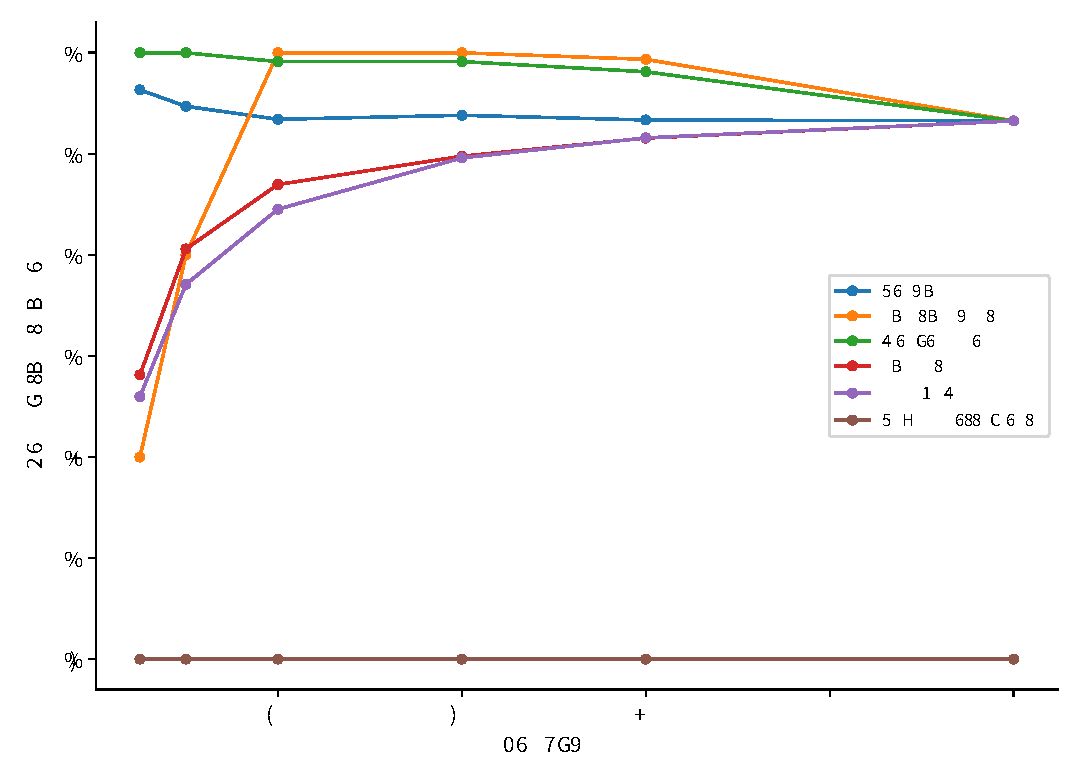
\includegraphics[width=\columnwidth]{figures/hcr_call_rate.pdf}
  \caption{不同调用预算下的有害修正率。学习式复检排序在低预算区间优于随机选择，接受门进一步减少高风险动作。}
  \label{fig:hcr-call-rate}
\end{figure}

提议动作未经接受门筛选时，最终 F1 随预算下降。5\% 和 20\% 预算下的 F1 分别为 0.9088 和 0.9015。60\% 和 100\% 预算下则为 0.8820 和 0.8660。调用增加会累积错误动作。加入接受门后，5\% 和 20\% 预算下的 F1 分别为 0.9117 和 0.9115。60\% 和 100\% 预算下均为 0.9115。表~\ref{tab:acceptance-budget} 汇总这四个预算点。基础工作点 B1 为 0.9118。有接受门的 0.9115 至 0.9117 与基线无统计差异，不能解释为数值不低于基线。图~\ref{fig:f1-call-rate} 显示，无接受门曲线随预算下降，双门控曲线保持在基线水平。

\begin{figure}[t]
  \centering
  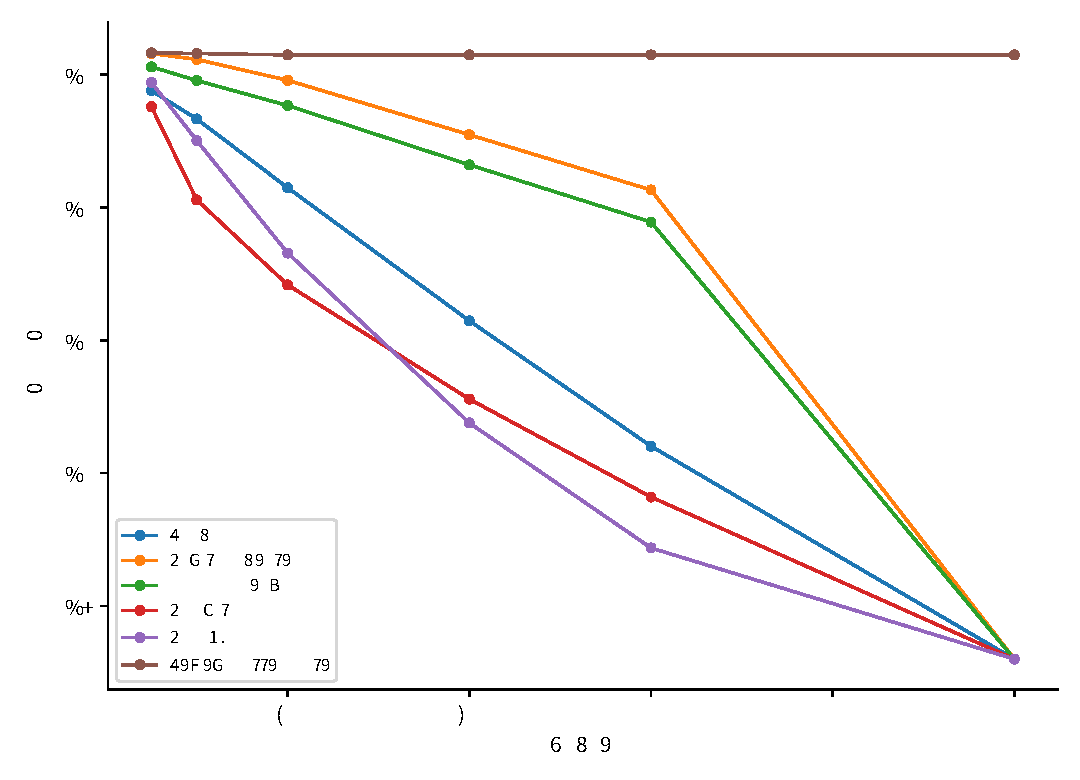
\includegraphics[width=\columnwidth]{figures/f1_call_rate.pdf}
  \caption{调用预算与最终 F1 的关系。缺少接受门时，增加调用会累积错误动作；采用接受门后，各预算点保持稳定。}
  \label{fig:f1-call-rate}
\end{figure}

\begin{table}[t]
  \centering
  \caption{接受门对预算曲线的影响}
  \label{tab:acceptance-budget}
  \begin{tabular}{ccc}
    \hline
    调用预算 & 无接受门 F1 & 有接受门 F1 \\
    \hline
    5\%   & 0.9088 & 0.9117 \\
    20\%  & 0.9015 & 0.9115 \\
    60\%  & 0.8820 & 0.9115 \\
    100\% & 0.8660 & 0.9115 \\
    \hline
  \end{tabular}
\end{table}

安全规则不消除推理成本。多模态验证器的单候选平均时延为 29.1 秒，P95 为 41.4 秒。调用预算从 5\% 增至 100\% 时，平均每图 token 消耗从 123 增至 2519，接近线性增长。100\% 调用对应最高成本，也在无接受门时产生最低 F1。复检门压缩调用量，接受门减少调用后的错误修改，二者分别作用于成本与风险。

端到端结果界定了双门控的作用范围。接受门将无门控方案的 HCR 从 0.9326 降至 0.4000，并把正确检测误删控制在 2 次。它没有完全阻断有害修正。有接受门的预算曲线保持在基线水平，但未证明检测精度提高。当前净收益仍受多模态验证器判断质量限制。系统因此把有限调用优先分配给高风险候选，并在训练证据不足时拒绝修改。
